\chapter{Regiones de Validación} \label{chap:ch6}

\newthought{En este capítulo} definiremos regiones de validación para verificar la normalización preliminar del fondo dominante $t\bar{t}$ obtenida en la CR estudiada en el capítulo anterior. Realizaremos una comparación de las simulaciones de MC corregidas con los datos en las VRs, reportando los resultados obtenidos en el número total de eventos y distribuciones.


\section{Definición de las regiones}

\begin{marginfigure}[5em]
    \subfloat[][\label{fig:ch6:BDTs:CR}]{\includegraphics[width=0.99\marginparwidth]{Assets/Plots/CR/h_mc16d_ttbar_ditau_bdt.eps}}\\
    \subfloat[][\label{fig:ch6:BDTs:SR}]{\includegraphics[width=0.99\marginparwidth]{Assets/Plots/SR/h_mc16d_ttbar_ditau_bdt.eps}}

    \caption{Distribuciones de $BDT$ del fondo simulado $t\bar{t}$ con los cortes de la región de control \subref{fig:ch6:BDTs:CR} y señal \subref{fig:ch6:BDTs:SR}, utilizados para definir la regiones de validación VR1 y VR2.}
    \label{fig:ch6:BDTs}
\end{marginfigure}

Como hemos discutido en los capítulos anteriores, en el presente análisis se utiliza el puntaje del BDT de identificación de los objetos DiTau como el principal corte de definición de las distintas regiones. Las CR del fondo $t\bar{t}$ en $BDT \leq -0.2$ y la SR preliminar en $BDT > 0.22$, resultan en un intervalo inutilizado en $-0.2 < BDT < 0.22$ en el que podemos colocar nuevas regiones.

Para verificar las estimaciones de los fondos y las correcciones que el factor de normalización $\mu_{t\bar{t}}$ introduce en el fondo $t\bar{t}$, definiremos dos regiones de validación, VR1 y VR2, basadas en distintas extrapolaciones entre la CR y la SR respectivamente, aunque con un nuevo rango de $BDT$ de los objetos DiTau incluidos. Obtenemos así una evolución progresiva de los cortes de selección. Para minimizar la presencia de señal en este primer conjunto de VRs, se optó por solo utilizar el intervalo $-0.2 < BDT < 0.0$, más alejado de la SR, como podemos observar en la \cref{fig:ch6:BDTs}.

Un resumen de las definiciones de las regiones VR1 y VR2 se encuentra en la \cref{tbl:ch6:VRs_definition}.

\begin{table*}[b]
    \small%
    \setlength{\tabcolsep}{1.2mm}%
    \begin{tabular}{L{40mm} L{30mm}L{30mm}L{30mm}L{30mm}}
\toprule
                                                    & \multicolumn{1}{c}{CR de $t\bar{t}$} & \multicolumn{1}{c}{VR1} & \multicolumn{1}{c}{VR2} & \multicolumn{1}{c}{SR} \\
\midrule                                         
Preselección                                        & $\checkmark$              & $\checkmark$              & $\checkmark$              & $\checkmark$              \\
$E_T^{\text{miss}}$                                 & $\geq \SI{50}{\GeV}$      & $\geq \SI{50}{\GeV}$      & ---                       & ---                       \\
$NJets$                                             & $\geq 2$                  & $\geq 2$                  & $\geq 3$                  & $\geq 3$                  \\
$NBJets$                                            & $\geq 2$                  & $\geq 2$                  & $\geq 1$                  & $\geq 1$                  \\
$\Delta R(\text{DiTau}, \text{Baseline Lepton})$    & $\geq 1.0$                & $\geq 1.0$                & $\geq 1.0$                & $\geq 1.0$                \\
$q_{\text{lead}} q_{\text{sublead}}$                & ---                       & ---                       & $-1$                      & $-1$                      \\
DiTau $BDT$                                         & $-1.0 \leq BDT \leq -0.2$ & $-0.2 \leq BDT \leq 0.0$  & $-0.2 \leq BDT \leq 0.0$  & $0.22 \leq BDT \leq 1.0$  \\
$NDiTau$                                            & 1                         & 1                         & 1                         & 1                         \\
\bottomrule
\end{tabular}
    \caption{Definiciones de las regiones de validación VR1 y VR2. Los cortes se aplican en el orden enlistado en la tabla. Los cortes en $NJets$ y $NBJets$ se realizan luego del OR entre (B)Jets y DiTaus ($\Delta R(\text{DiTau}, \text{(B)Jet}) > 1$).}
    \label{tbl:ch6:VRs_definition}
\end{table*}



\begin{figure}[t]
    \hspace{2em}
    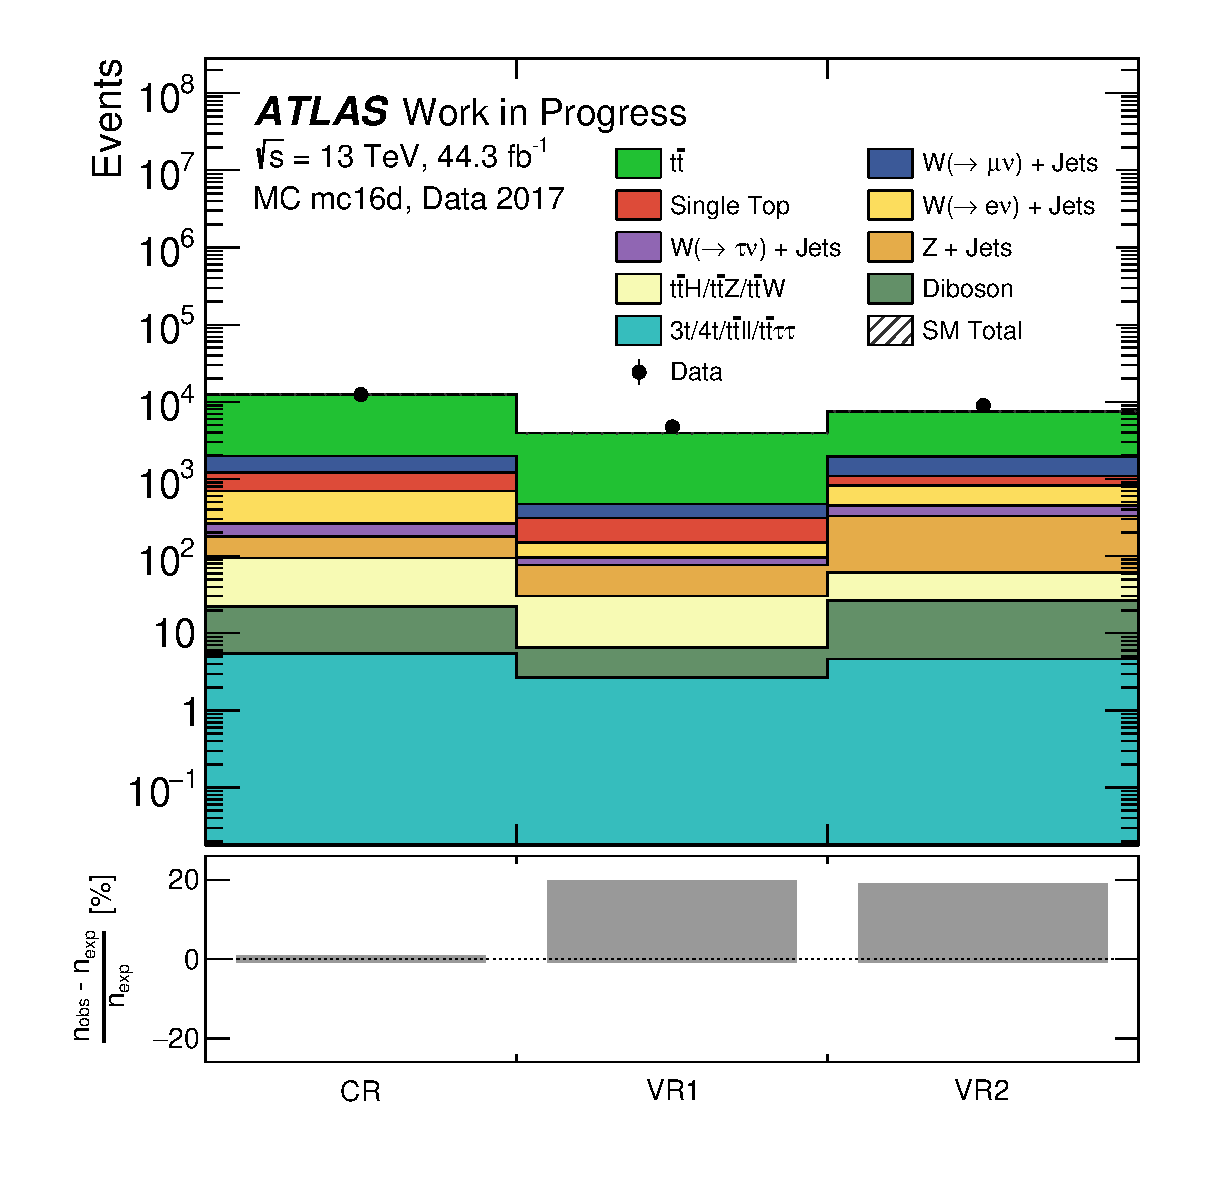
\includegraphics[width=0.75\linewidth]{Assets/Plots/h_mc16d_data17_delta.eps}
    \caption[][-1em]{Diferencias porcentuales en el número de total eventos de fondo simulados respecto a los datos en las regiones de validación, utilizando los factores de normalización $\mu_{t\bar{t}}$ calculados en el \cref{tbl:ch5:ttbar_mu}.}
    \label{fig:ch6:VRs_results}
    \setfloatalignment{b}
\end{figure}

\begin{table}[t]
    \small%
    \centering%
    \begin{tabular}{L{27mm} C{22mm}C{22mm}C{22mm}}
\toprule
                                & CR de $t\bar{t}$  & VR1               & VR2               \\
\midrule
Fondo SM                        & 13835.938         & 4361.346          & 8246.951          \\
Fondo SM con $\mu_{t\bar{t}}$   & 12475.000         & 3914.042          & 7524.113          \\
Datos                           & 12474             & 4694              & 8971              \\
$\Delta$                        & 0.00\%            & 19.92\%           & 19.22\%           \\
\bottomrule
\end{tabular}
    \caption{Número total de eventos y diferencias porcentuales ($\Delta$) entre eventos simulados del SM y los datos experimentales en las regiones de validación VR1 y VR2. Solo se incluyen incertezas estadísticas y del factor de transferencia $\mu_{t\bar{t}}$. Trabajo en progreso.}
    \label{tbl:ch6:VRs_results}
    \setfloatalignment{b}
\end{table}

\section{Resultados en la región de validación}

Los resultados obtenidos en las regiones de validación VR1 y VR2 se resumen en la \cref{fig:ch6:VRs_results} y en la \cref{tbl:ch6:VRs_results}. Ambas regiones de validación presentan una discrepancia entre el número total de eventos en los datos y en los fondos simulados del SM del 19.92\% y 19.22\% respectivamente, en ambos casos con un defecto de los eventos de MC.

A fin de investigar el origen de esta discrepancia, se procedió al análisis de las distribuciones de momento transverso en los leptones, jets y ditaus en las regiones de validación VR1 y VR2, mostradas en las \cref{fig:ch6:VRs_distributions,fig:ch6:VRs_distributions_2}. Se observa una mayor diferencia entre las simulaciones de MC y los datos en los objetos de menor $p_T$. Esto puede deberse a la falta del fondo Multijet, que aun no ha sido incluido en el análisis y suele contribuir a la reconstrucción de leptones \textit{fake} a bajo $p_T$.

Estas diferencias exceden las incertezas estadísticas consideradas en las distribuciones de los procesos simulados. Sin embargo, es importante recordar que no se han considerado en este trabajo las incertezas sistemáticas originadas en la generación de los eventos y en la reconstrucción y calibración de los objetos físicos incluidos en el análisis, ni su posible correlación en las distintas regiones de control y validación. Si suponemos una incerteza sistemática de las simulaciones MC aproximada de $\sigma_b = 20\% \cdot b$, donde $b$ es el número de eventos de fondo en la región, las discrepancias en el número total de eventos resultan inferiores a una desviación estándar en todas las regiones de validación.



\clearpage{}
\begin{figure*}[th!]
    \centering
    \setlength{\individualPlotWidth}{0.434\fulllinewidth}
    %
    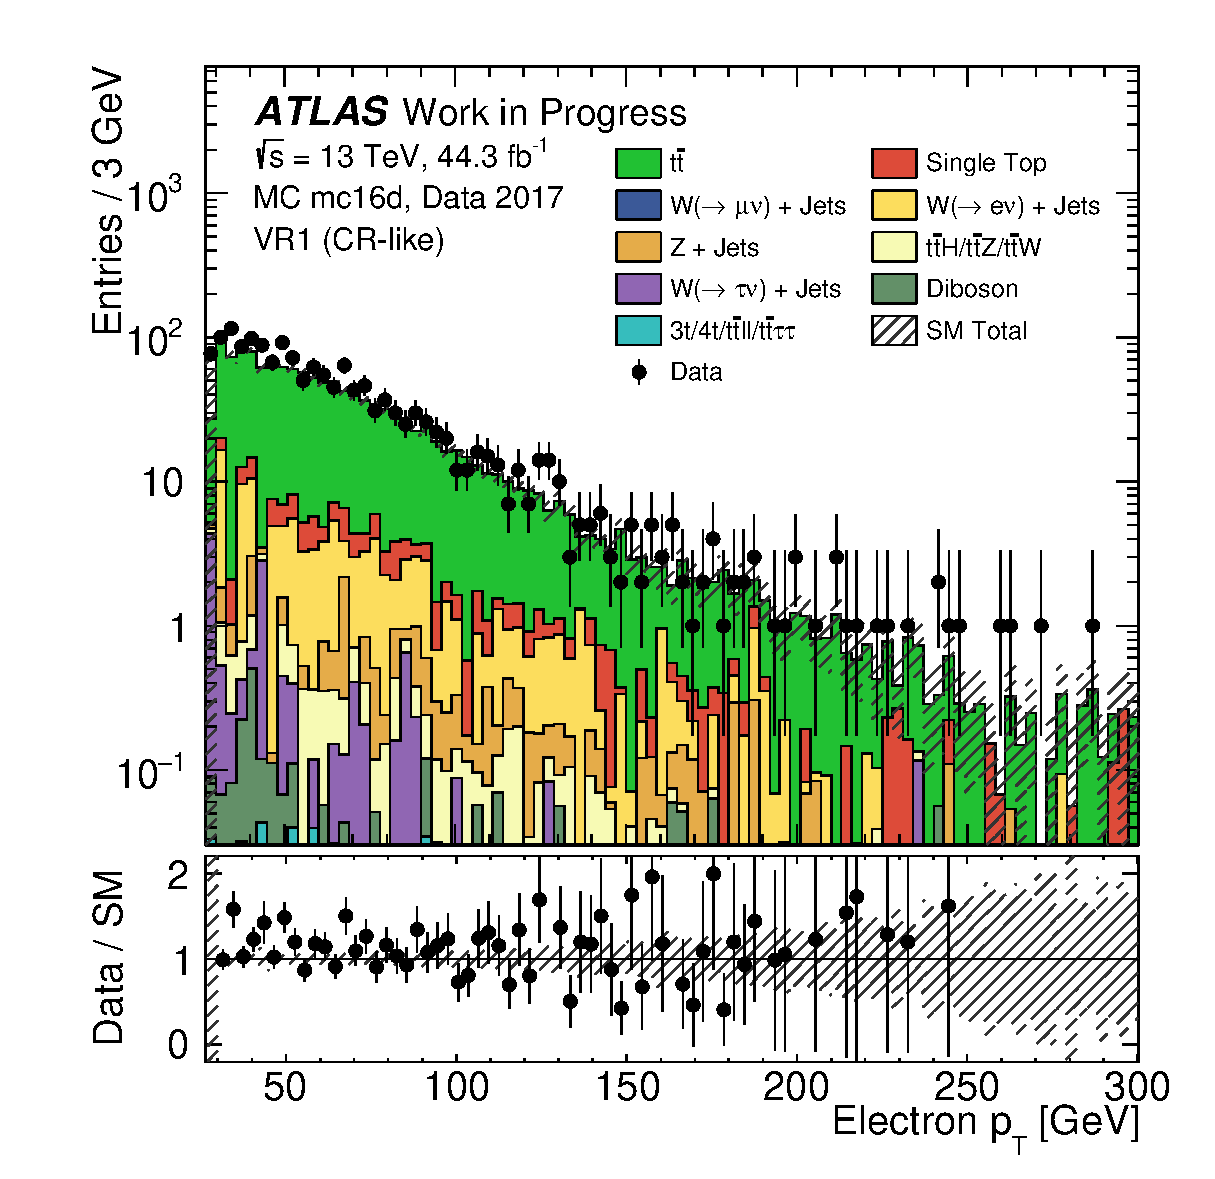
\includegraphics[width=\individualPlotWidth]{Assets/Plots/VR1/h_stack_mc16d_data17_el_pt.eps}
    \hspace{1em}
    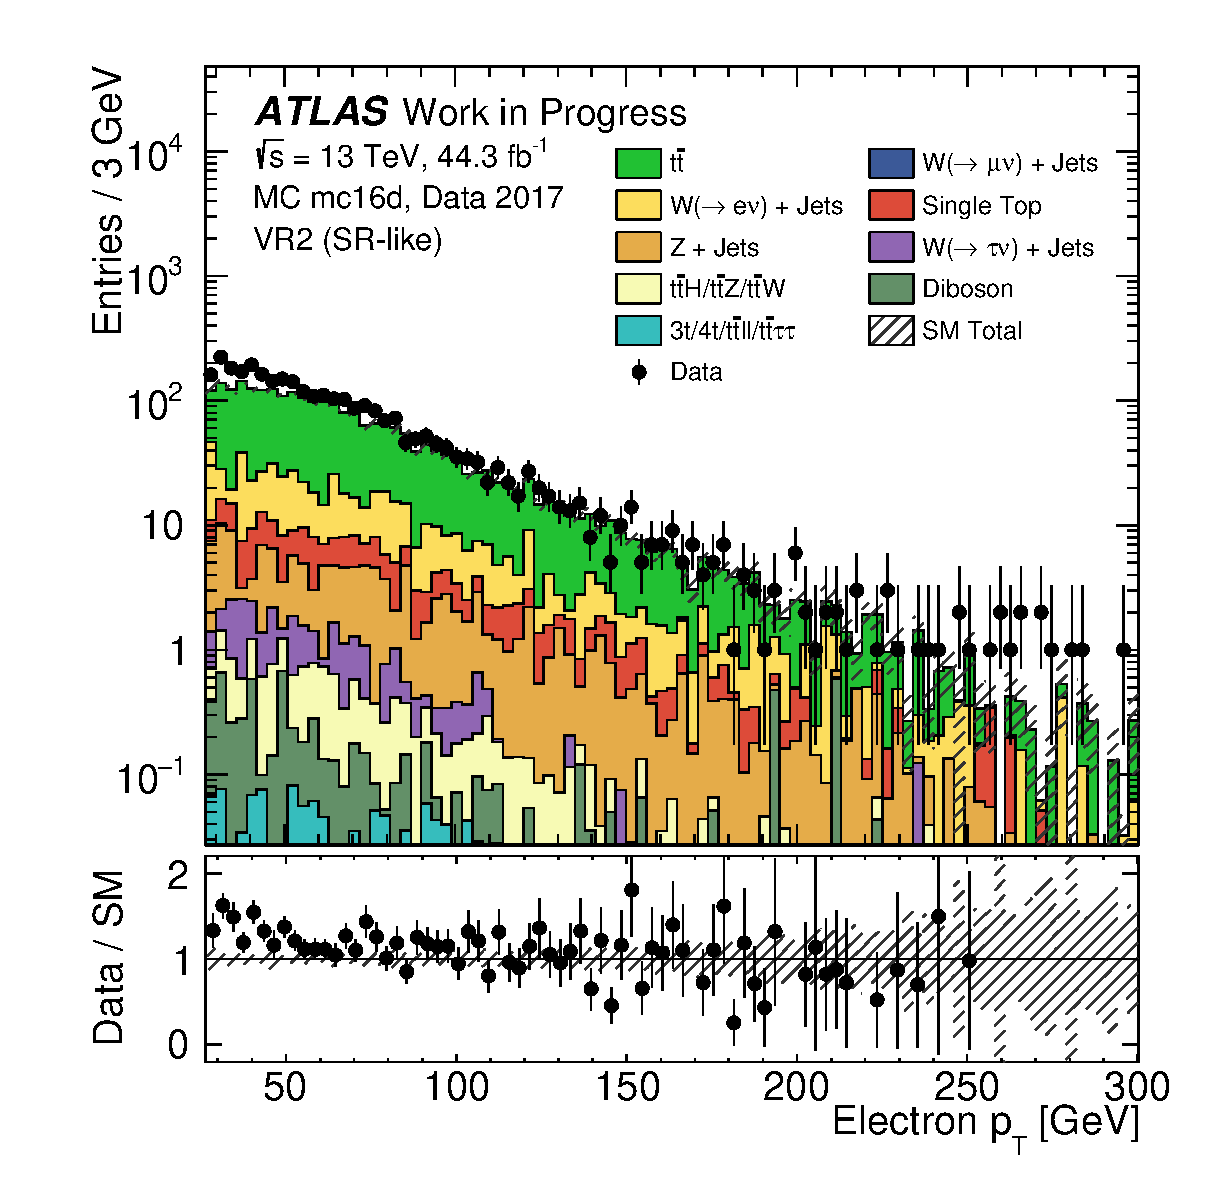
\includegraphics[width=\individualPlotWidth]{Assets/Plots/VR2/h_stack_mc16d_data17_el_pt.eps}

    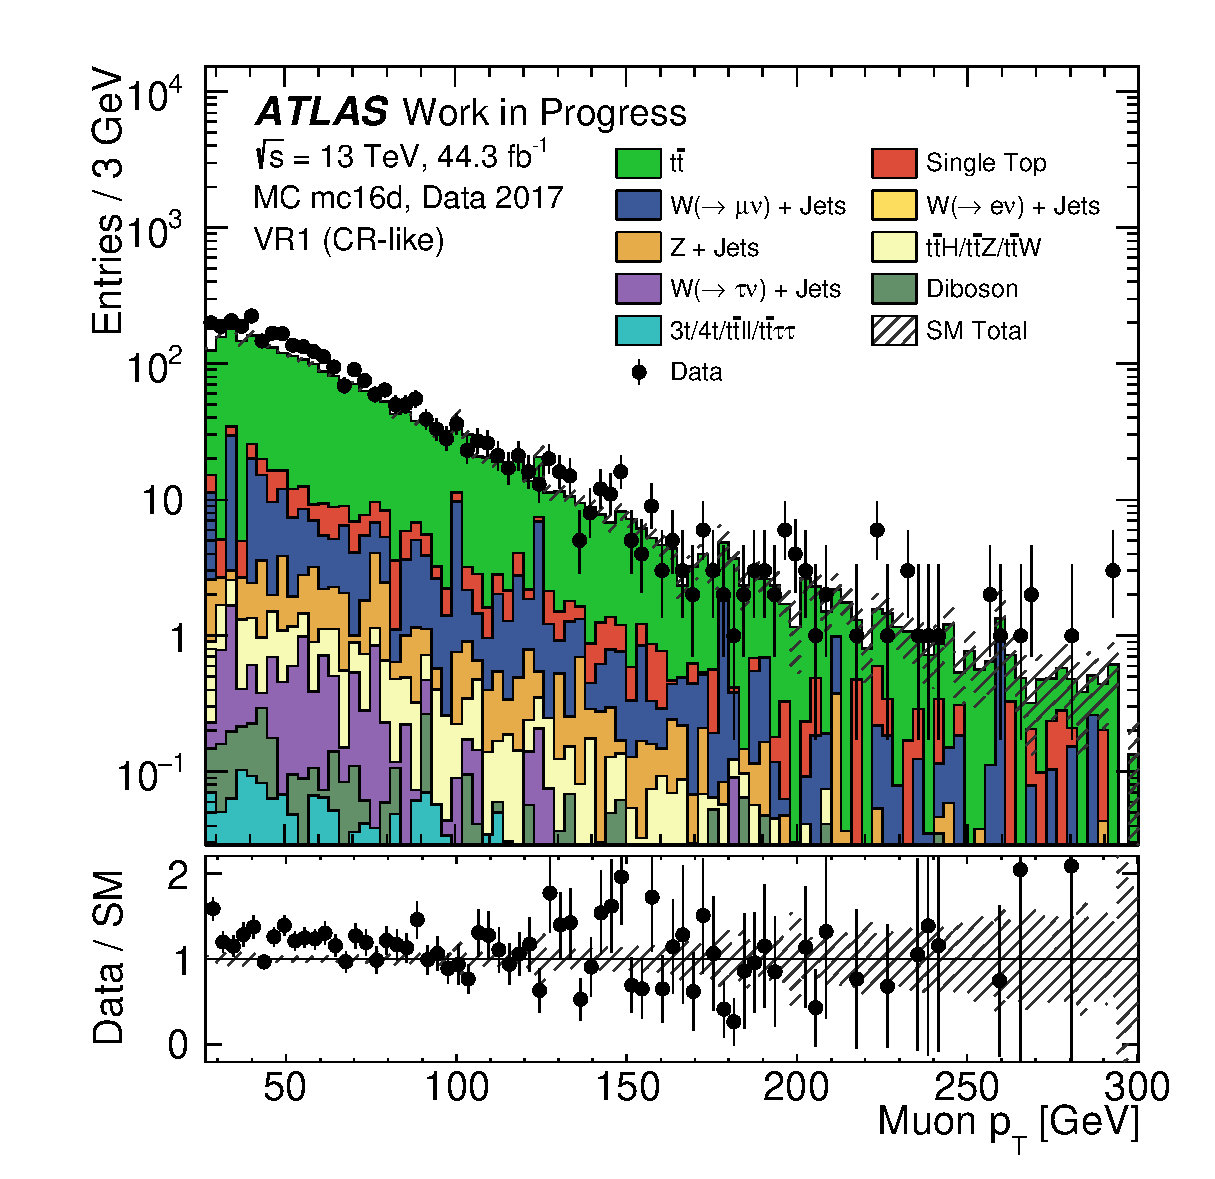
\includegraphics[width=\individualPlotWidth]{Assets/Plots/VR1/h_stack_mc16d_data17_mu_pt.eps}
    \hspace{1em}
    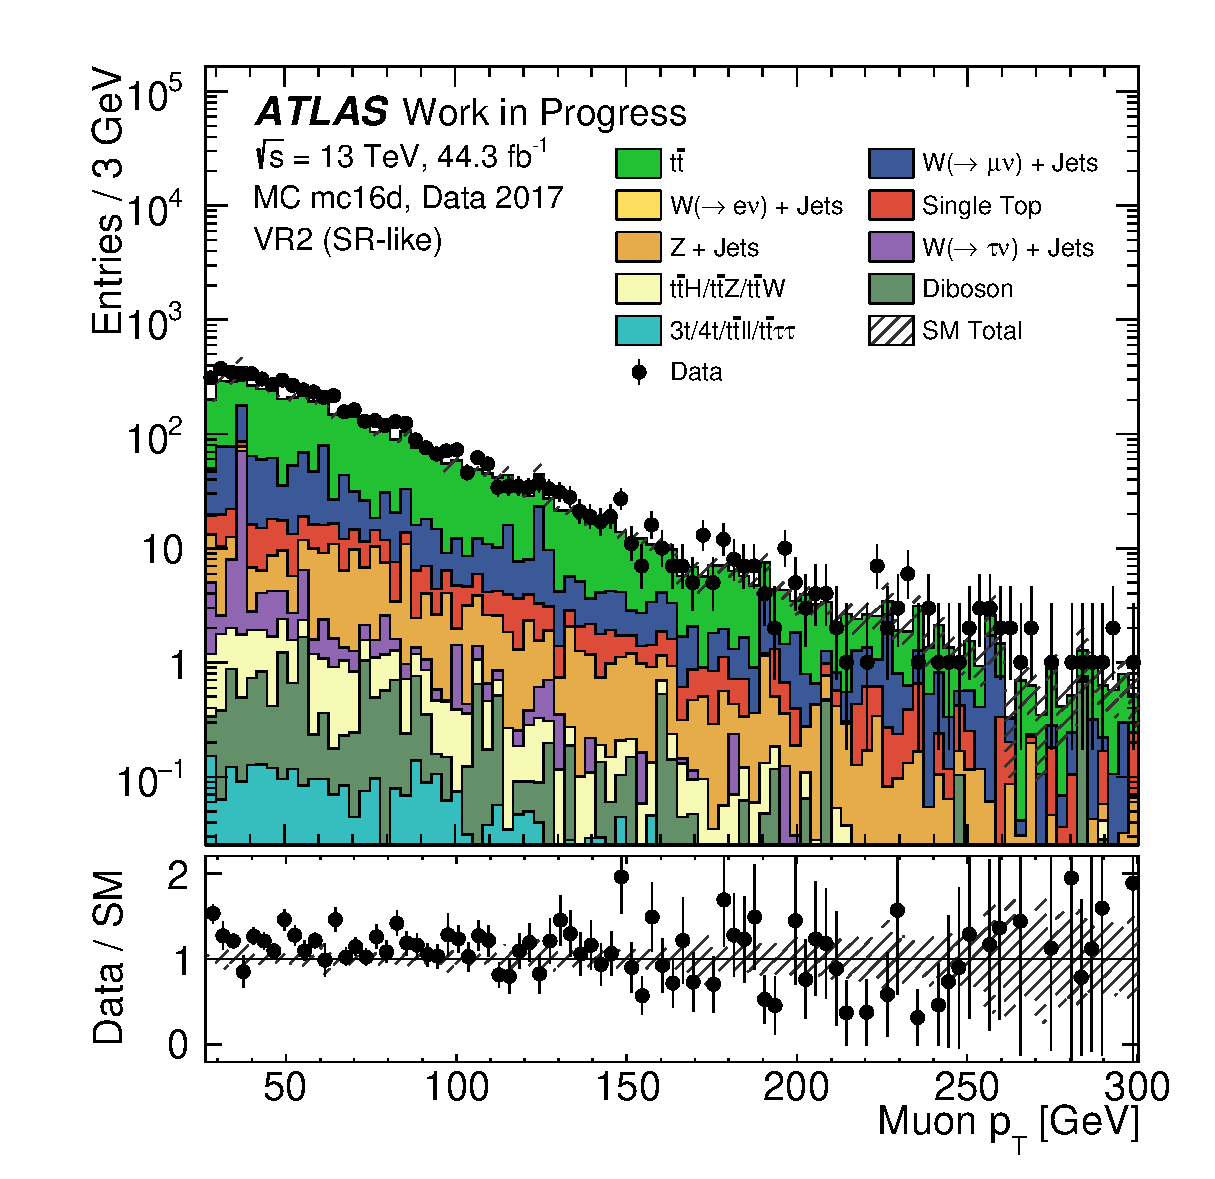
\includegraphics[width=\individualPlotWidth]{Assets/Plots/VR2/h_stack_mc16d_data17_mu_pt.eps}

    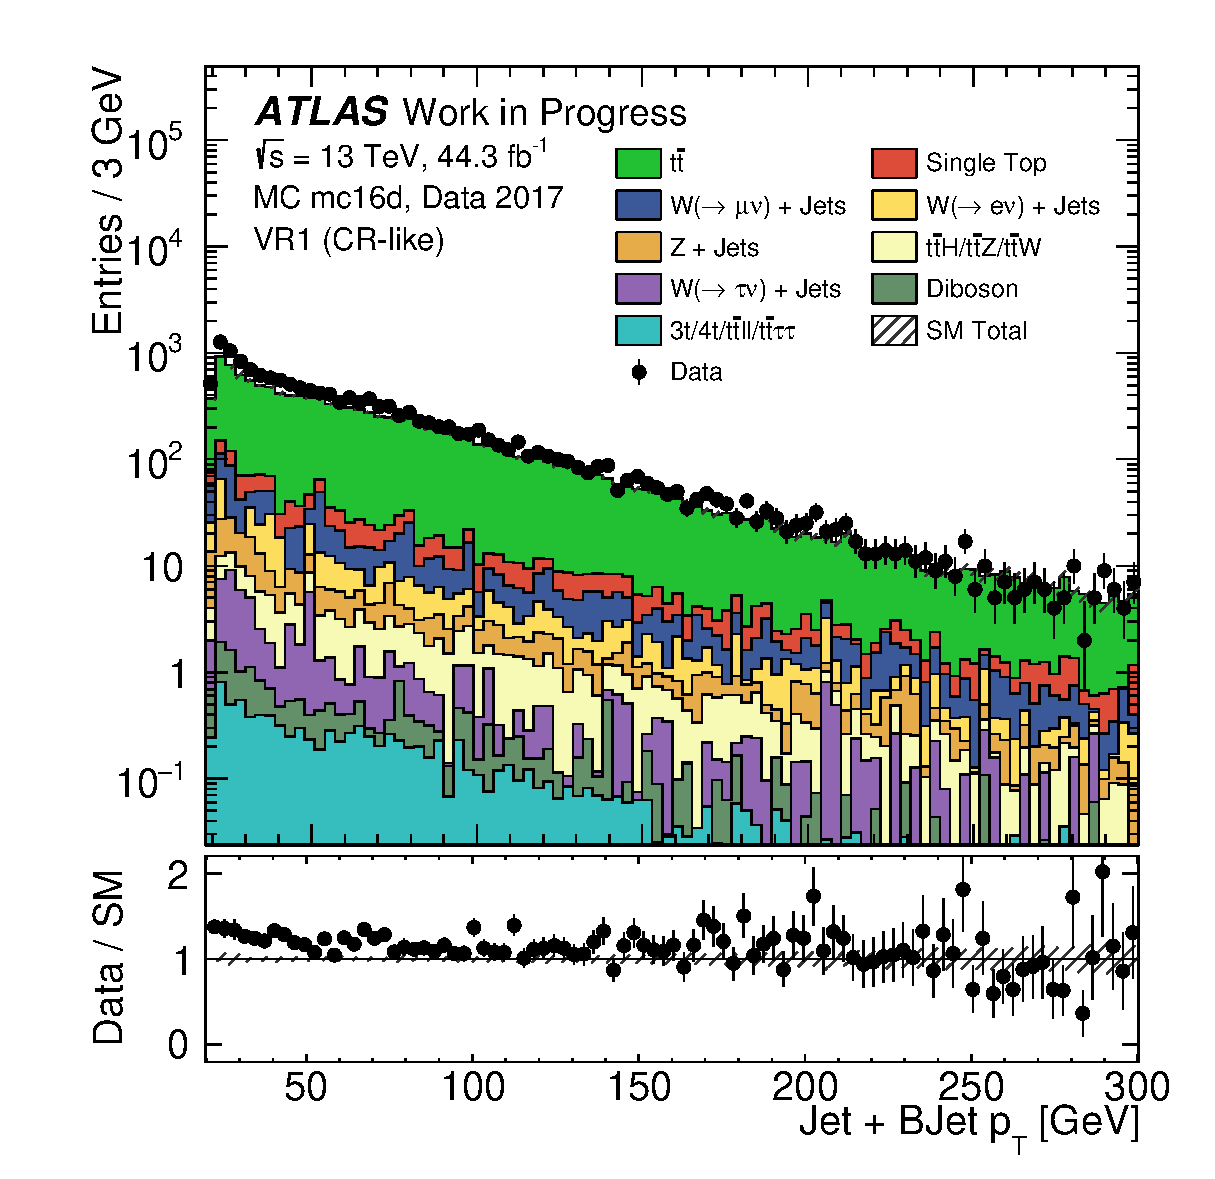
\includegraphics[width=\individualPlotWidth]{Assets/Plots/VR1/h_stack_mc16d_data17_jet_tot_pt.eps}
    \hspace{1em}
    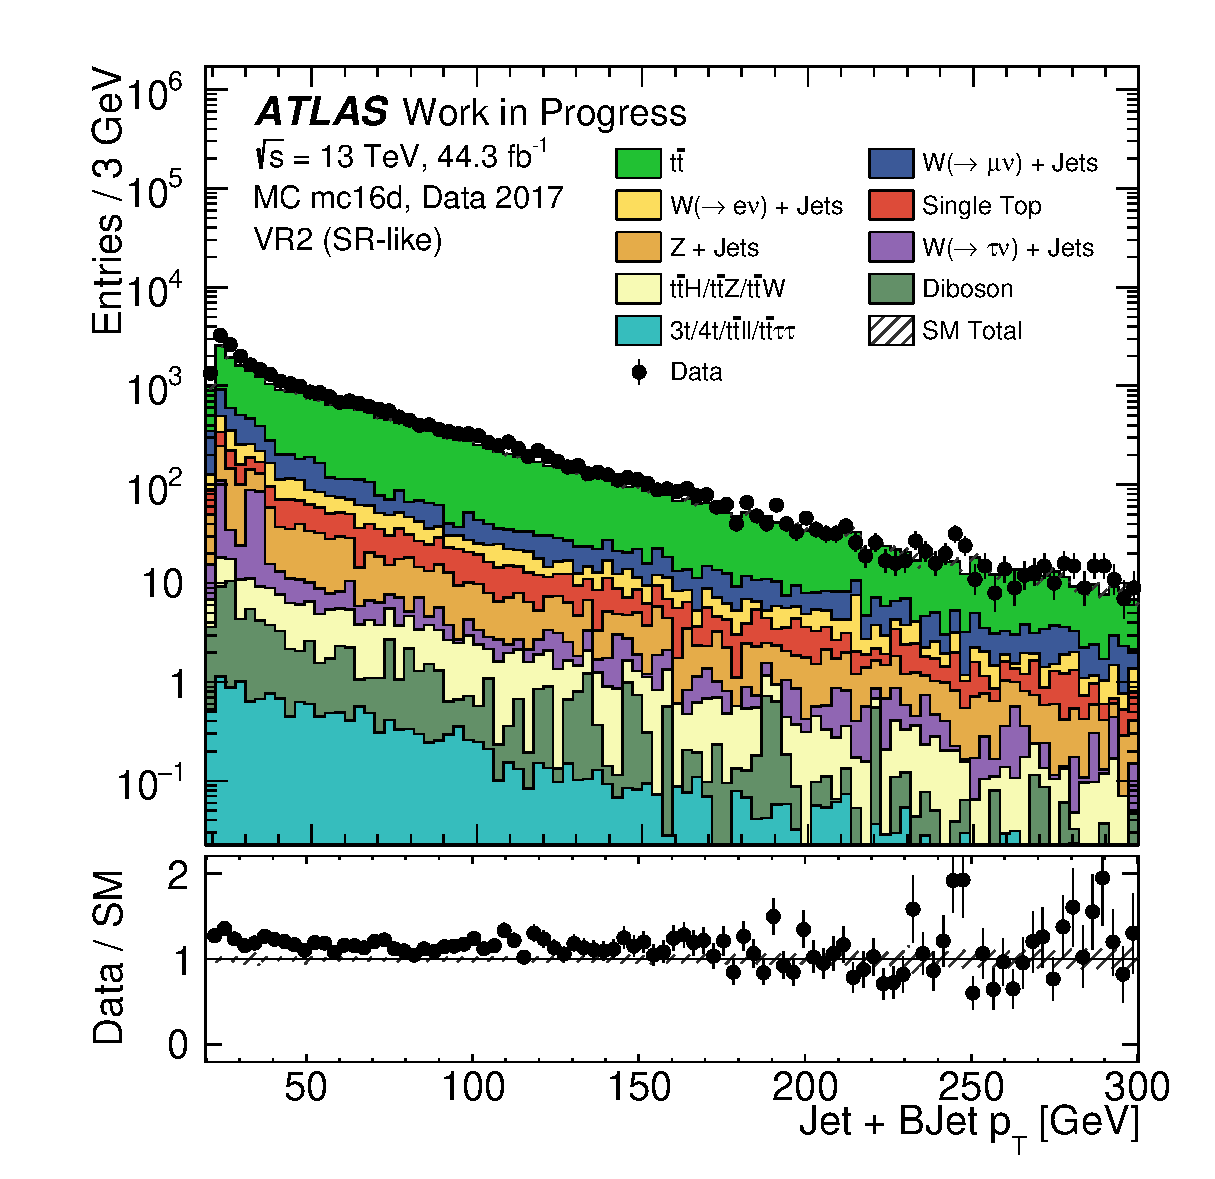
\includegraphics[width=\individualPlotWidth]{Assets/Plots/VR2/h_stack_mc16d_data17_jet_tot_pt.eps}

    \fullwidthCaption{Distribuciones cinemáticas de $p_T$ de los leptones, (b)jets y DiTaus en las regiones de validación VR1 (izquierda) y VR2 (derecha).}
    \label{fig:ch6:VRs_distributions}
\end{figure*}

\clearpage{}
%\let\oldthefigure\thefigure % This make latex crash... but not needed
% since it was already used in ch5...
%\renewcommand{\thefigure}{\oldthefigure \ (Cont.)}
\begin{figure*}[th!]
    \centering
    \setlength{\individualPlotWidth}{0.434\fulllinewidth}
    %
    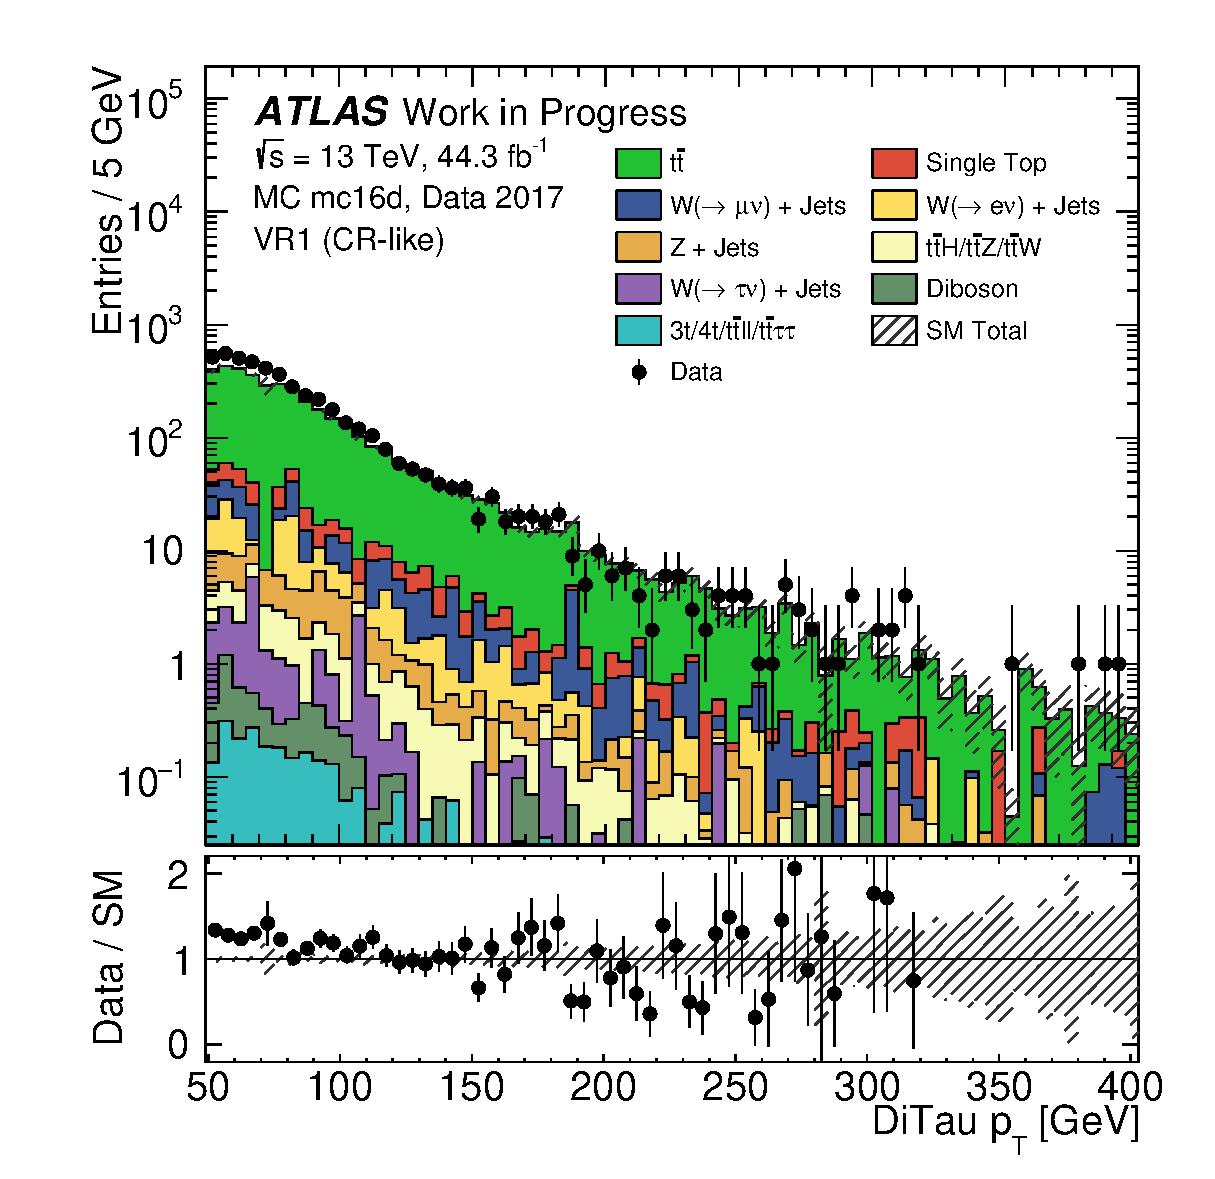
\includegraphics[width=\individualPlotWidth]{Assets/Plots/VR1/h_stack_mc16d_data17_ditau_pt.eps}
    \hspace{1em}
    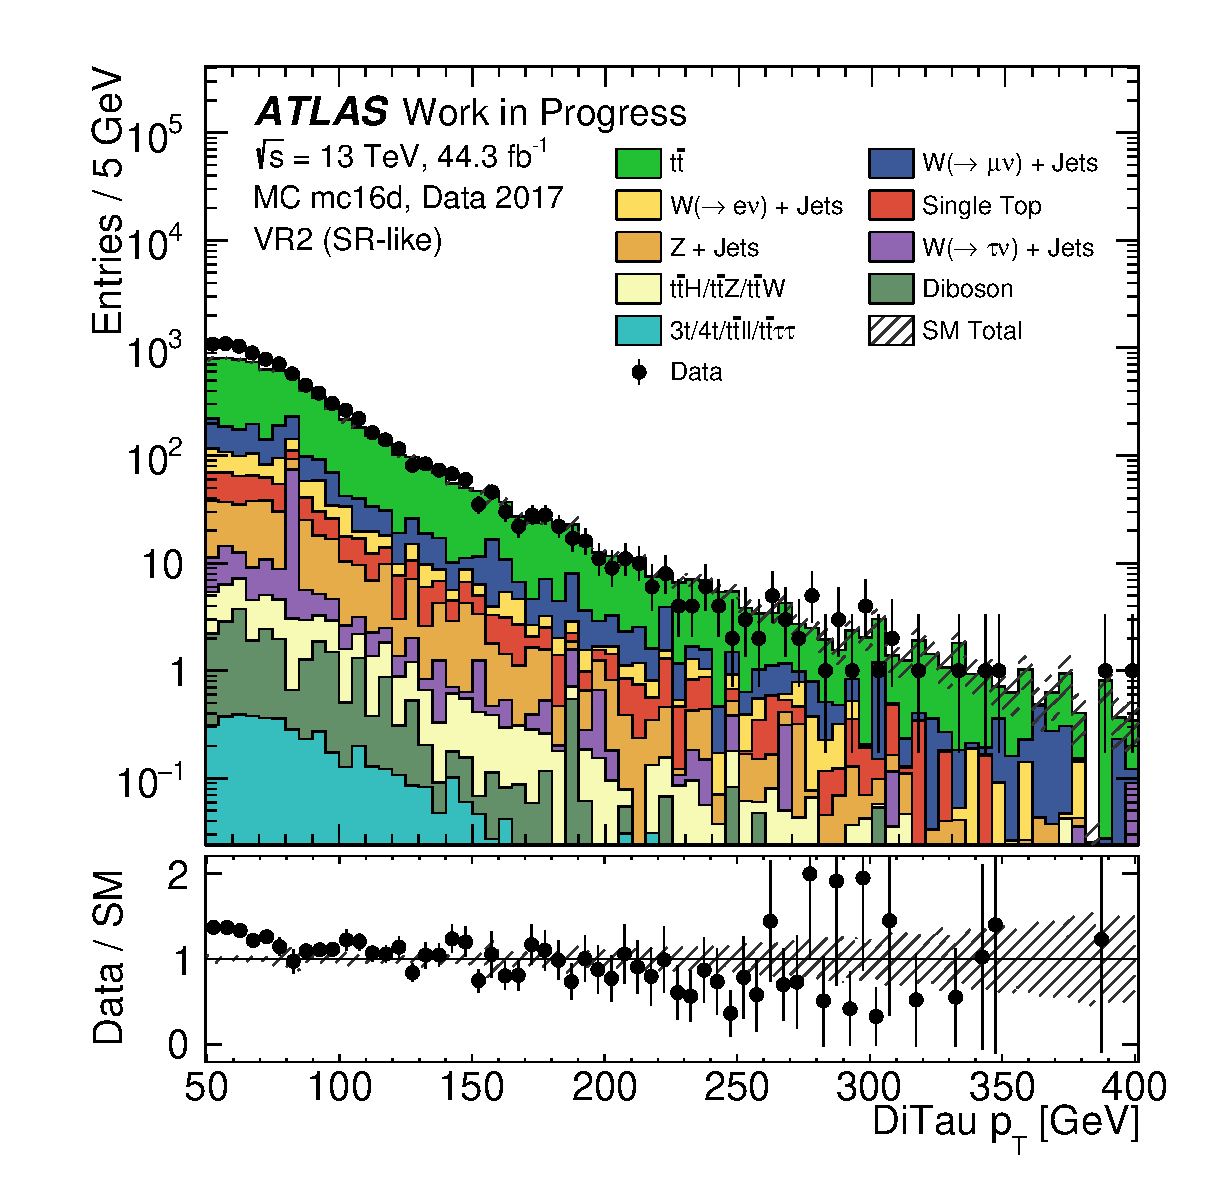
\includegraphics[width=\individualPlotWidth]{Assets/Plots/VR2/h_stack_mc16d_data17_ditau_pt.eps}

    \fullwidthCaption{Distribuciones cinemáticas de $p_T$ de los leptones, (b)jets y DiTaus en las regiones de validación VR1 (izquierda) y VR2 (derecha).}
    \label{fig:ch6:VRs_distributions_2}
    %\ContinuedFloat
\end{figure*}
%\renewcommand{\thefigure}{\oldthefigure}

\cleardoublepage{}